% Options for packages loaded elsewhere
\PassOptionsToPackage{unicode}{hyperref}
\PassOptionsToPackage{hyphens}{url}
%
\documentclass[
  ignorenonframetext,
]{beamer}
\usepackage{pgfpages}
\setbeamertemplate{caption}[numbered]
\setbeamertemplate{caption label separator}{: }
\setbeamercolor{caption name}{fg=normal text.fg}
\beamertemplatenavigationsymbolsempty
% Prevent slide breaks in the middle of a paragraph
\widowpenalties 1 10000
\raggedbottom
\setbeamertemplate{part page}{
  \centering
  \begin{beamercolorbox}[sep=16pt,center]{part title}
    \usebeamerfont{part title}\insertpart\par
  \end{beamercolorbox}
}
\setbeamertemplate{section page}{
  \centering
  \begin{beamercolorbox}[sep=12pt,center]{part title}
    \usebeamerfont{section title}\insertsection\par
  \end{beamercolorbox}
}
\setbeamertemplate{subsection page}{
  \centering
  \begin{beamercolorbox}[sep=8pt,center]{part title}
    \usebeamerfont{subsection title}\insertsubsection\par
  \end{beamercolorbox}
}
\AtBeginPart{
  \frame{\partpage}
}
\AtBeginSection{
  \ifbibliography
  \else
    \frame{\sectionpage}
  \fi
}
\AtBeginSubsection{
  \frame{\subsectionpage}
}
\usepackage{amsmath,amssymb}
\usepackage{lmodern}
\usepackage{iftex}
\ifPDFTeX
  \usepackage[T1]{fontenc}
  \usepackage[utf8]{inputenc}
  \usepackage{textcomp} % provide euro and other symbols
\else % if luatex or xetex
  \usepackage{unicode-math}
  \defaultfontfeatures{Scale=MatchLowercase}
  \defaultfontfeatures[\rmfamily]{Ligatures=TeX,Scale=1}
\fi
% Use upquote if available, for straight quotes in verbatim environments
\IfFileExists{upquote.sty}{\usepackage{upquote}}{}
\IfFileExists{microtype.sty}{% use microtype if available
  \usepackage[]{microtype}
  \UseMicrotypeSet[protrusion]{basicmath} % disable protrusion for tt fonts
}{}
\makeatletter
\@ifundefined{KOMAClassName}{% if non-KOMA class
  \IfFileExists{parskip.sty}{%
    \usepackage{parskip}
  }{% else
    \setlength{\parindent}{0pt}
    \setlength{\parskip}{6pt plus 2pt minus 1pt}}
}{% if KOMA class
  \KOMAoptions{parskip=half}}
\makeatother
\usepackage{xcolor}
\newif\ifbibliography
\setlength{\emergencystretch}{3em} % prevent overfull lines
\providecommand{\tightlist}{%
  \setlength{\itemsep}{0pt}\setlength{\parskip}{0pt}}
\setcounter{secnumdepth}{-\maxdimen} % remove section numbering
\ifLuaTeX
  \usepackage{selnolig}  % disable illegal ligatures
\fi
\IfFileExists{bookmark.sty}{\usepackage{bookmark}}{\usepackage{hyperref}}
\IfFileExists{xurl.sty}{\usepackage{xurl}}{} % add URL line breaks if available
\urlstyle{same} % disable monospaced font for URLs
\hypersetup{
  pdftitle={Simulation Based Methods for Network Inference},
  pdfauthor={Marthyna Luiza WEBER},
  hidelinks,
  pdfcreator={LaTeX via pandoc}}

\title{Simulation Based Methods for Network Inference}
\author{Marthyna Luiza WEBER}
\date{2023-05-15}
\institute{Grenoble INP - Ensimag}

\begin{document}
\frame{\titlepage}

\begin{frame}
\tableofcontents
\end{frame}

\hypertarget{initial-definitions}{%
\section{Initial definitions}\label{initial-definitions}}

\begin{frame}{1. Partial Correlation}
\protect\hypertarget{partial-correlation}{}
Correlation coefficient between \(X_1\) and \(X_2\) after removing the
influence of \(Y\), accounting for the scaling of the variables.

\begin{itemize}
\tightlist
\item
  Partial covariance: The partial covariance between \(X_1\) and \(X_2\)
  with reference to \(Y\) is calculated with:
\end{itemize}

\[
Cov(X_1, X_2 \cdot Y) = \mathbb{E}[(X_1 - \hat{X}1(Y))(X_2 - \hat{X}2(Y))]
\]

\begin{itemize}
\tightlist
\item
  \(\hat{X}_l(Y)\) is the projection of \(X_l\) on \(Y\), which is the
  expected value of \(X_l\) given \(Y\):
\end{itemize}

\[
\hat{X}_l(Y) = \mathbb{E}(X_l)+\frac{Cov(X_l,Y)}{Var(Y)}(Y-\mathbb{E}(Y))
\]
\end{frame}

\begin{frame}{1. Partial correlation}
\protect\hypertarget{partial-correlation-1}{}
\begin{itemize}
\tightlist
\item
  Lemma:
  \[ Cov(X_\mathit{l},X_\mathit{m}\cdot Y) = Cov(X_\mathit{l},X_\mathit{m}) - Cov(X_\mathit{l},Y)Var(Y)^{-1}Cov(X_\mathit{m}Y)^T \]
  \small Given a vector \(\mathbf{X} = (X_1, \ldots, X_p)\) of \(p\)
  random variables. We have:
\end{itemize}

\[ Cov^{\text{partial}}(\mathbf{X}_{\mathit{l,m}}) = Cov(X_\mathit{l},X_\mathit{m}\cdot X_{\mathit{V\backslash\{l,m\}}}) \]

\begin{itemize}
\tightlist
\item
  Partial correlation:
  \[ \rho^{\text{partial}}(\mathbf{X}_{\mathit{l,m}})=\frac{Cov(X_\mathit{l},X_\mathit{m}\cdot X_{\mathit{V\backslash\{l,m\}}})}{\sqrt{Var(X_\mathit{l} \cdot X_{\mathit{V\backslash\{l,m\}}}) Var(X_\mathit{m} \cdot X_{\mathit{V\backslash\{l,m\}}})}} \]
\end{itemize}
\end{frame}

\begin{frame}{2. Regular vines}
\protect\hypertarget{regular-vines}{}
\small A vine in which two edges in tree \(T_i\) are joined by an edge
in tree \(T_{i+1}\) only if these edges share a common node.

\begin{columns}[T]
  \begin{column}{.5\textwidth}
    \centering
    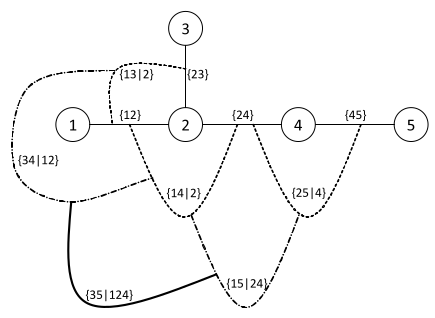
\includegraphics[width=1.1\textwidth]{regular_vine.png}
  \end{column}
  \begin{column}{.5\textwidth}
    \begin{itemize}
      \item Constraint set $U_e$: variables reachable from edge $e$
      \item Conditioning set $D_e$: variables shared between $U_e$ and edge adjacent to $e$ in the next tree
      \item Conditioned set $\{C_{1e}, C_{2e}\}$: symmetric difference of $U_e$ and $D_e$
    \end{itemize}
  \end{column}
\end{columns}

\begin{itemize}
\tightlist
\item
  \(\{L|K\}\): the constraint set, with conditioned set \(L\) and
  conditioning set \(K\).
\end{itemize}
\end{frame}

\begin{frame}{4. C-vines}
\protect\hypertarget{c-vines}{}
\begin{itemize}
\tightlist
\item
  \small C-vines: vines where each tree \(T_i\) has a unique node of
  degree \(d-i\)
\item
  \small D-vines: vines where each node in \(T_i\) has a degree at most
  2.
\end{itemize}

\begin{columns}[T]
  \begin{column}{0.5\textwidth}
    \centering
    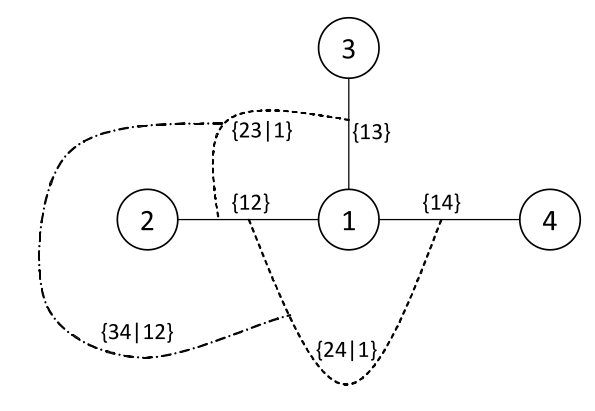
\includegraphics[width=\textwidth]{c-vines.png}
    \tiny A C-vine
  \end{column}
  \begin{column}{0.5\textwidth}
    \centering
    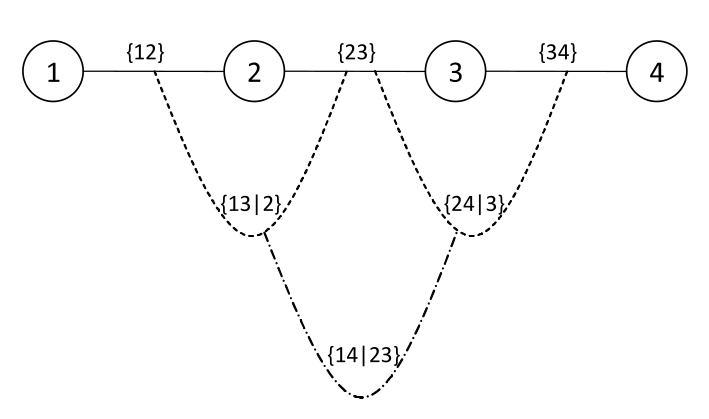
\includegraphics[width=\textwidth]{d-vines.png}
    \tiny A D-vine
  \end{column}
\end{columns}
\end{frame}

\begin{frame}{5. Generatating random correlation matrices with C-vines}
\protect\hypertarget{generatating-random-correlation-matrices-with-c-vines}{}
Algorithm to generate a random correlation matrix \(\boldsymbol{R}\)
with density proportional to \(det(\boldsymbol{R})^{\eta-1}\), with
\(\eta > 1\):

\begin{enumerate}
    \item Initialize $\beta = \eta + \frac{d-1}{2}$
    \item Loop for $k = 1, \ldots, d-1$:
    \begin{enumerate}
        \item $\beta = \beta - \frac{1}{2}$
        \item Loop for $i = k+1, \ldots, d$:
        \begin{enumerate}
            \item generate $p_{k,i;1,\ldots,k-1}$ $\sim$ Beta$(\beta, \beta)$  on $(-1,1)$
            \item use the recursive formula for partial correlations calculation
        \end{enumerate}
    \end{enumerate}
    \item Return $\boldsymbol{R}$, a $d \times d$ correlation matrix
\end{enumerate}
\end{frame}

\end{document}
